\section{Grundlagen}
\subsection{Industrie 4.0}
Hier steht etwas zur Industrie 4.0



\subsection{Digitaler Zwilling}
Digitale Zwillinge im industriellen Kontext nehmen eine zunehmend zentralle Rolle ein und das Interesse ist in den letzten Jahren immer mehr gestiegen.
Erstmals wurde das Konzept von M. Grieves im Jahr 2003 in einer Präsentation zum Product Lifecycle Management vorgestellt \cite{DTGrieves}. 
Grieves definierte drei zentrale Komponenten, die zusammen das Informationsmodell des digitalen Zwilling bilden:
\begin{itemize}
    \item ein reales Objekt in der physischen Welt,
    \item ein digitales Abbild dieses Objekts in einem virtuellen Raum, sowie
    \item eine Schnittstelle, die den Informationsfluss zwischen diesen beiden ermöglicht.
\end{itemize}

Auf Basis des von Grieves entwickelten Informationsmodells hat sich der Begriff des digitalen Zwillings stetig weiter entwickelt und in verschiedenen Bereichen Einzug erhalten. 
Aufgrund der verschiedenen Fachgebiete und unkonsister Definitionen des digitalen Zwillings haben sich in der Vergangenheit unterschiedliche Ausprägungen des Begriffs des digitalen Zwillings gebildet.
Diese unterscheiden sich insbesondere in der Tiefe der Datenintegration zwischen dem physischen Objekt und seinem virtuellen Abbild.
Während ein einfacher digitaler Zwilling lediglich ein einfaches Modell mit statischen Daten ist, ermöglichen fortgeschrittene Zwillinge einen bidrektionalen Datenaustausch zwischen physischem und virtuellem Objekt. 

Grundsätzlich lassen sich digitale Zwilling nach Typ und Instanz unterscheiden.
Typen sind allgemeine Abbilder, die grundlegende Eigenschaften und Verhaltensmodelle einer Produktgruppe beschreiben. 
Sie können mit einer Klasse in der Softwarentwicklung verglichen werden, die als Vorlage für konkrete Instanzen dienen.
Typen können zum Beispiel einen bestimmten Maschinentyp hinsichtlich Aufbau, Stuktur oder Schnittstellen beschreiben, ohne dabei Bezug zu einer einzelnen physischen Maschine zu nehmen.
Instanzen wiederrum sind einzigartig, und beschreiben ein konkretes Produkt, wie zum Beispiel eine Maschine, die einzigartig über eine Seriennummer identifizierbar ist.
Häufig sind Instanzen Aussprägungen eines Types mit einer Verbindung zu einem realen Objekt, wodurch beispielsweise die Überwachung des Zustands einer Maschine ermöglicht wird.
Analog zur Softwarentwicklung können diese als instanziiertes Objekt einer Klasse gesehen werden. \cite{ZEISS}

Drei wesentliche Konzepte, die immmer wieder im Zusammenhang des digitalen Zwillings gleichbedeutend gennant werden sind das digitale Modell, der digitale Schatten und der digitale Zwilling. \cite{KRITZINGER20181016}
Die Klassifizierung nach der Art des Informationsfluss ist hierbei nur für Instanzen des digitalen Zwillings sinnvoll.
Sie unterscheiden sich dabei wesentlich in der Art des Informationsflusses.
Digitale Modelle sind statische Abbilder physischer Objekte, haben jedoch keine Verbindung zu diesen. 
Oft werden sie zur Veranschauclichung oder Konstruktion genutzt, wie zum beispiel ein 3D-Modell einer Maschine.
Zwar können reale Daten, wie etwa Maße oder Materialeigenschaften einer Anlage oder Maschine in ein solches Modell integriert werden, allerdings erfolgt die Eingabe dabei immmer manuel.
Änderungen an dem realen Objekt werden nicht automatisch aktualisiert und bleiben somit ohne Einfluss auf das digitale Modell.
Der digitale Schatten ergänzt das digitale Modell um eine unindirektionale Verbindung zum realen Objekt.
Dabei fließen Daten des physischen Objekts meist in Echtzeit über zum Beispiel geeignete Sensoren zum digitalen Objekt.
Der Schatten bildet den aktuellen Zustand des Objekts ab, hat aber keine Rückkoplung zu diesem.
Ein typisches Beispiel für einen digitalen Schatten wäre das Condition Monitoring, wobei der Zustand einer Maschine mit geeigneten Sensoren abgebildet wird.
Mit einer aktiven Rückkoplung zum realen Objekt wird der digitale Schatten zum digitalen Zwilling.
Es entsteht eine Feedback-Schleife und erlaubt dem virtuellen Objekt Einfluss auf das reale System zu nehmen.

% Quelle: file:///C:/Users/Heinke/Documents/Bachelorarbeit/02%20Literatur/Digitaler_Zwilling/Klassifizierung_DT.pdf

\begin{figure}[htbp]
    \centering
    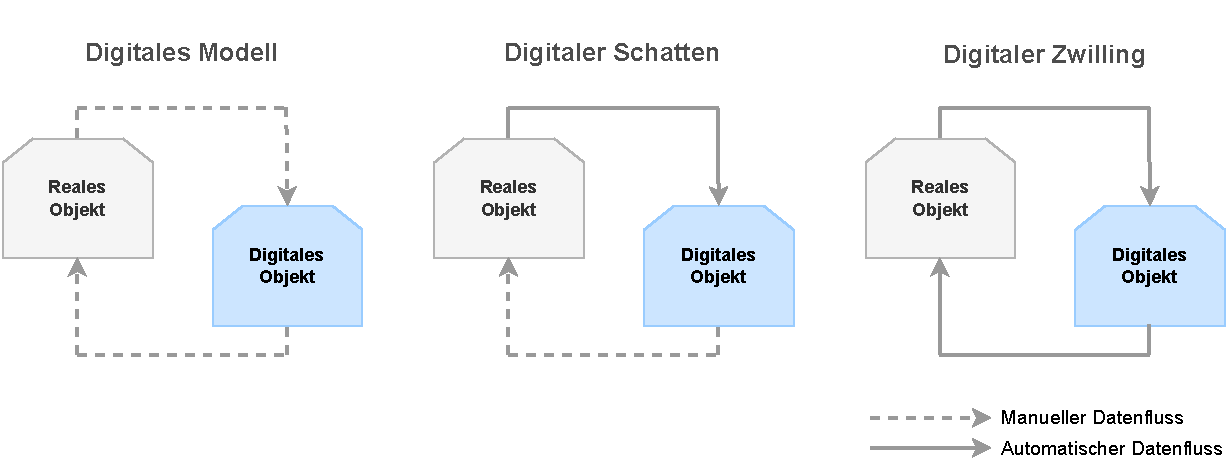
\includegraphics[width=1\textwidth]{Bilder/klassifizierung_DT.pdf}
    \caption{Klassifizierung des DT}
    \label{fig:klassifizierungDT}
\end{figure}

% Digitales Modell, digitaler Schatten und digitaler zwilling


% Definition nach Stark und Damerau des DT: 

% A digital twin is a digital representation of an active unique product (real device, object, machine, service, or intangible asset) or unique product-service system (a system consisting of a product and a related service) that comprises its selected characteristics, properties, conditions, and behaviors by means of models, information, and data within a single or even across multiple life cycle phases.

% \url{https://link.springer.com/referenceworkentry/10.1007/978-3-642-35950-7_16870-1#citeas}


\subsection{Asset Administration Shell}
Die Verwaltungsschale (engl. Asset Administration Shell) ist ein Schlüsselkonzept innerhalb des Referenzarchitekturmodell Industrie 4.0 \cite{RAMI4.0}. Sie bildet die Grundlage für die Umsetzung und Entwicklung interoperabler digitaler Zwillinge im industriellen Umfeld.
Das Konzept wurde maßgeblich von der Plattform Industrie 4.0 entwickelt und erstmlas im Jahr 2016 als Teil von RAMI 4.0 eingeführt.
% Das Architekturmodell ist ein Leitfaden für die Industrie und dient als Hilfestellung um die digitale Transformation in einem Unternehmen systematisch umzusetzten.
% Es soll helfen, die komplexen Anforderungen an die Industrie 4.0 für die Allgemeinheit verständlich zu machen.

Innerhalb von RAMI 4.0 ist die Verwaltungsschale eine virtuelle Hülle um ein Asset und repräsentiert dieses digital.
Sie enthält dabei alle relevanten Daten, Eigenschaften und Funktionen eines Assets über den gesamten Lebenszyklus hinweg.
Enthalten sind diese Informationen dabei in unterschiedlichen Submodellen, die immer einen bestimmten Aspekt eines Assets abbilden. 
Durch die standardisierte Struktur bildet die Verwaltungsschale die Grundlage für einen einheitlichen Informationsaustausch über System -und Unternehmensgrenzen hinweg.

Die Umsetzung und Weiterentwicklung der Verwaltungsschale wird seit 2020 von der Industrial Digital Twin Association (IDTA) organisiert und gesteuert.
Ziel der IDTA ist es den digitalen Zwilling auf Basis der Verwaltungsschale zu standardisieren und in Form von Open Source Softwarelösungen in das industrielle Umfeld zu integrieren.
Die Verwaltungsschale wird in verschiedenen Spezifikationen der IDTA dokumentiert und stetig weiterenwickelt.
Aktuell bildet die AAS Version 3 den neuesten Entwicklungsstand und ist ebenfalls die Basis für diese Arbeit.

Verwaltungsschalen represäntieren immer genau ein Asset und müssen global eindeutig identifizierbar sein.
In der Industrie können Assets physische Objekte, wie eine Anlage oder eine Maschine sein oder aber auch virtuelle Elemente wie Software oder eine Idee.
In RAMI 4.0 wird davon ausgegangen, das Assets immmer einen konkreten Nutzen für ein Unternehmen bzw. eine Organisation bieten.
Zusammen mit der Verwaltungsschale wird ein Asset zur sogenannten Industrie 4.0 Komonente. 

\begin{figure}[htbp]
    \centering
    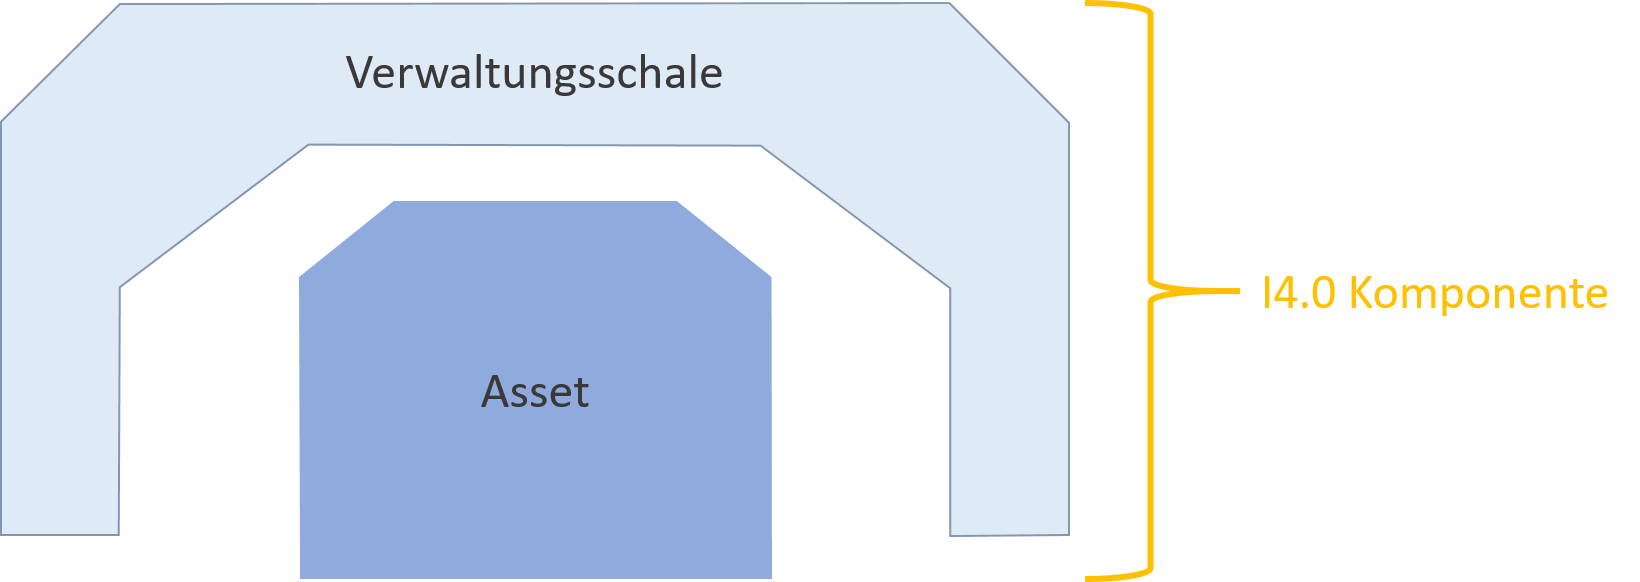
\includegraphics[width=0.7\textwidth]{Bilder/aas.png}
    \caption{Industrie 4.0 Komponente}
    \label{fig:klassifizierungDT}
\end{figure}

Der Austausch von Informationen über die Verwaltungsschale kann auf unterschiedliche Weise erfolgen.
Die einfachste Möglichkeit ist der Austausch über Dateien. Hierfür gibt es speziell für die AAS entwickelte AASX-Dateien, die einen einfachen Austausch statischer Verwaltungsschalen erlauben.
Typ-2 Verwaltungsschalen hingegen werden von einer Laufzeitumgebung gehosted und ermöglichen dadurch einen dynamischen Zugriff auf Informationen.
Über definierte Schnittstellen (APIs) können Daten aus der Verwaltungsschale gelesen oder geschrieben werden.
Die fortschrittlichste Form ist die Peer-to-peer Kommunikation, bei der I4.0-Komponenten eigenständig über die I4.0-Sprache miteinander kommunizioeren können.
[IDTA Specification Part3a] 

Allgemein kann zwischen Typ -und Instanz-Verwaltungsschalen unterschieden werden.
Typ-AAS beschreiben allgemeine Eigenschaften eines Produkttyp wie einen bestimmten Maschinen-Typ, während Instanz-Verwaltungsschalen immer einem spezifischen Objekt zugeordnet werden.
Typen können zum Besipiel allgemeine Dokumente zu einer bestimmten Maschinenart enthalten.
Abgeleitet davon kann eine Instanz für eine ausgelieferte Maschine erstellt werden, die beispielsweise über die Seriennummer oder den Aufenthaltsort eindeutig identifizierbar wird.

Bestimmte Aspekte eines Assets werden in verschiedenen Submodellen verwaltet.
Man kann sich dies wie ein Schubladensystem vorstellen, wobei jede Schublade einen bestimmten Bereich des Assets abdeckt.
In einer Schublade könnten zum Beispiel technische Dokumentationen liegen und in einer Anderen Typenschilder. 
Genau wie die AAS müssen diese Teilmodelle global eindeutig identifizierbar sein.
Ein Teilmodell besteht dabei immmer aus verschiedenen Submodellelementen - dazu zählen zum Beispiel Eigenschaften, Operationen oder auch Dateien.
Es ist wichtig alle Submodelle bzw. alle Elemente über eine eindeutige Semantik zu beschreiben.
Hierfür gibt es sogenannte "Concept Desciptions".
Sie helfen bei der Klassifizierung von Daten und sorgen für ein gemeinsames Verständnis unterschiedlicher Systeme.
Diese Beschreibungen können entweder direkt in die AAS eingebetet werden oder über externes Standards wie zum Beispiel ECLASS referenziert werden.
ECLASS basiert auf dem Datenmodell der Norm IEC 61360 [IEC 61360], welche eine standardisierte Struktur für Merkmale und deren semantische Beschreibung definiert.
Ein vereinfachtes SChema des Metamodells der Verwaltungsschale ist nachfolgend in Abbildung 3 dargestellt.  [Spezifikation Metamodell
]

\begin{figure}[htbp]
    \centering
    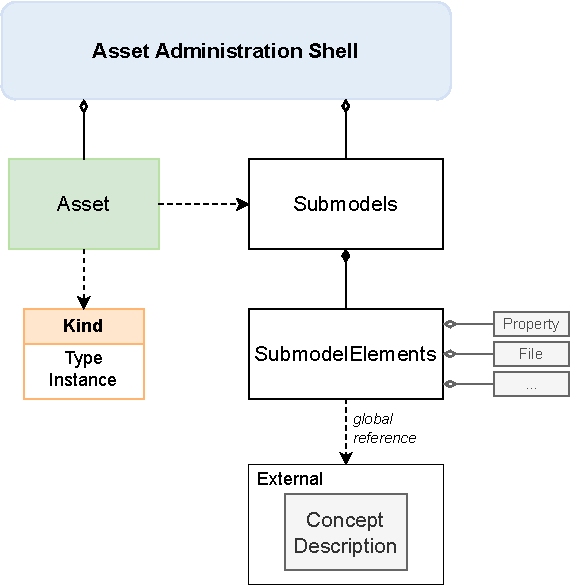
\includegraphics[width=0.7\textwidth]{Bilder/Metamodel.pdf}
    \caption{Metamodell der AAS}
    \label{fig:klassifizierungDT}
\end{figure}

Um die Erstlleung solcher Submodelle zu erleichtern und gleichzeitig Interoperabilität zu gewährleisten, stellt die IDTA standardisierte Submodellvorlagen - sogenannte Submodel Templates - zur Verfügung.
Aktuell sind 34 dieser Templates veröffentlicht, viele weitere sind in der Entwicklung oder im Überprüfungsprozess und werden in Zukunft ergänzt.
Die bereits verfügbaren Templates enthalten unteranderem Submodelle wie das digitale Typenschild oder den Carbon Footprint.
Alle Eigenschaften innerhalb dieser Vorlagen werden dabei in Verbindung mit dem ECLASS-Standard einheiltich semantisch beschrieben.
Diese Templates könen über ein zentrales Repository bezogen werden und bilden die Basis für eine interoperable semantische Datenstruktur.
Außerdem 


\subsection{Digitaler Produktpass}
Der digitale Produtpass (DPP) ist ein zentrales Instrument der Europäischen Union zur Umsetzung einer nachhaltigen, digitalen Transformation.
Das Konzept des digitalen Produktpasse wurde erstmals im Rahmen des European Green Deal von der Europäischen Kommission im Jahr 2019 vorgestellt [Quelle: https://eur-lex.europa.eu/legal-content/EN/TXT/?uri=CELEX:52019DC0640] und mittlerweile im Zuge der Eco Design for Sustainable Products Regulation (ESPR) [Quelle] als verpflichtendes Mittel eingeführt.
Ziel ist es, die Transparenz über ökologische Merkmale von Produkten wie verwendete Materialien, Recylcebarkeit oder die CO2-Bilanz deutlich zu verbessern.

Als erstes soll der digitale Produktpass im Jahr 2027 für Batterien eingeführt werden. Weitere Produktkategorien werden in den nächsten Jahren folgen.
Dabei kann der Produktpass als eine digitale Akte gesehen werden, die produktspezifische Daten über den gesamten Lebenszyklus aufzeichnet.
Gefordert werden wird zum Beispiel die Implementierung eines digitalen Typenschildes auf Basis von IEC 61406 oder die Bereitstellung des Product Carbon Footprints entlang des gesamten Lebenszyklus eines Produktes.



Hier muss noch die technologische Umsetzung (mit AAS) hin.


Bezug zu AAS nehmen...
\subsection{Künstliche Intelligenz im industriellen Kontext}



\subsection{robcoell}
Was ist die robocell? Wodurch zeichnet sie sich aus?

Eingehen auf das Füllmodul


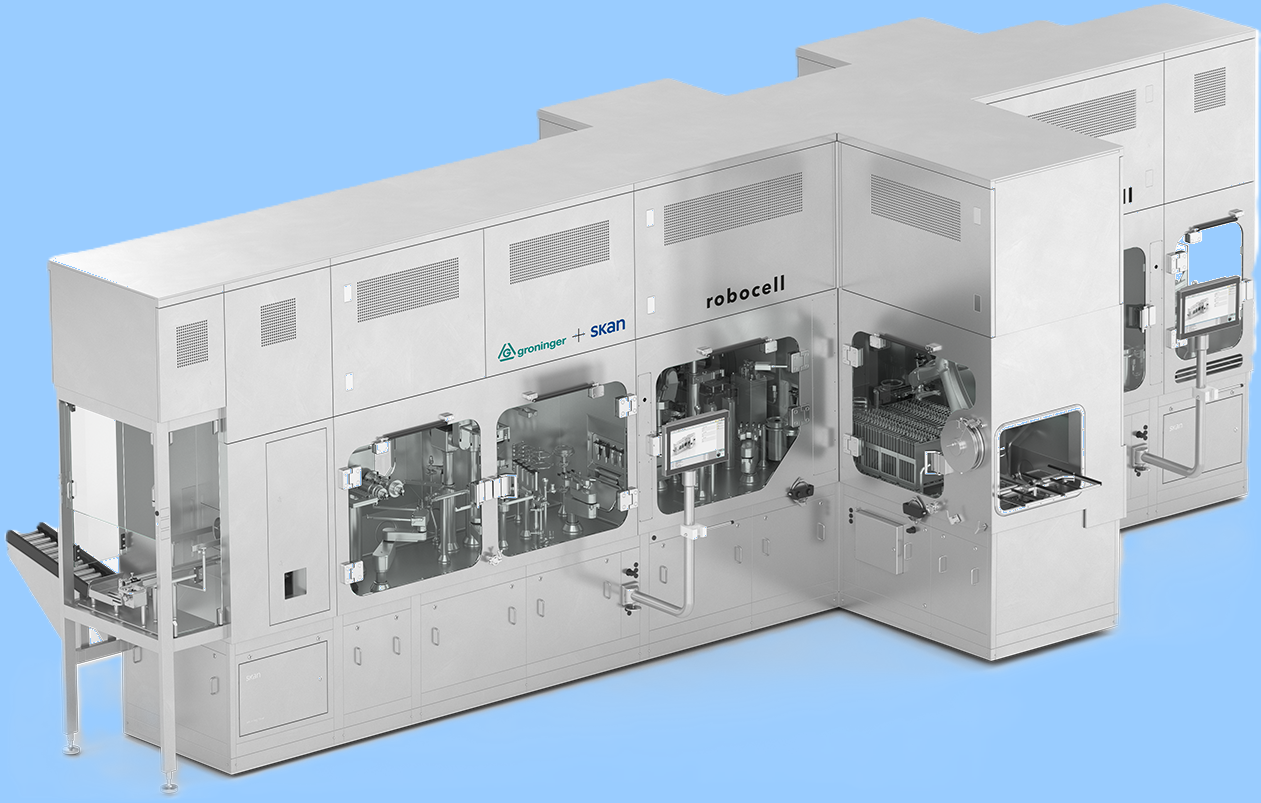
\includegraphics{Bilder/robocell_FS2_rgb_Logo.png}
\subsection{Technologische Grundlagen}
Brauche ich das?
\subsubsection{AASX Package Exlporer}
\subsubsection{OPC UA}
\subsubsection{Basyx}